%% This document shows an example of writing exam paper in a main file, and 5 separate questions file.
%%
\documentclass[12pt]{article}
%\usepackage{finalxm}
\usepackage[minutes]{finalxm}
%\usepackage[answers]{finalxm}
\usepackage{pdflscape}	% for landscape layout on specific page 
%
% Declare graphics path 
% \graphicspath{{./figs/}}	% a subfolder named figs

%%%%%%%%%%%%%%%%%%%%%%%%
%%% SETUP TITLE PAGE %%%
%%%%%%%%%%%%%%%%%%%%%%%%
\mtefe{Akhir} 			% Akhir, Pertengahan
\semester{Kedua}		% Pertama, Kedua
\sidang{2017/2018}		
\examMonthYear{Jun 2018}
\courseCode{ENT390}
\courseNameEn{Bioinstrumentation 1}
\courseNameBM{Bioinstrumentasi 1}
\pagesbm{TIGA PULUH SATU}	% used if the number of pages exceeds 30
\durationhr{2 Jam}		% duration of exam
\makeatletter 
\if@minutes
	\durationmin{30 Minit}	% MUST be enabled using \usepackage[minutes]{finalxm}
\fi 		
\makeatother		

\begin{document}
% cover page

%\begin{titlepage}	
\makecover

\instructionen{
	This question paper has \textbf{TWO (2)} parts. Answer \textbf{all} questions in \mbox{\textbf{Part A}} and \mbox{\textbf{THREE (3)}} question in \mbox{\textbf{Part B}}. Each question contributes 25 marks.%
}
\instructionbm{%
	Kertas soalan ini mengandungi \textbf{DUA (2)} bahagian. Jawab \textbf{semua} soalan di \mbox{\textbf{Bahagian A}} dan \mbox{\textbf{TIGA (3)}} soalan di \mbox{\textbf{Bahagian B}}. Setiap soalan menyumbang 25 markah.%
}

%\end{titlepage}

%%%%%%%%%%%%%%%%%%%%%%%%%%%%
%%% MAIN BODY START HERE %%%
%%%%%%%%%%%%%%%%%%%%%%%%%%%%
\setmainstyle

% PART A
\newpartenx{Answer all questions} 

\newpartbm{Jawab semua soalan}
\bigskip

% Question 1
\question

\listbeginx	% start 1st level question
	\item \label{chemical} What chemical reactions you expect to see at these electrodes? 
	
	\translation{Apakah tindak balas kimia yang anda jangka dapat dilihat pada kedua –dua elektrod} 
	
	\qmarks{4}	% define marks
	
	\item A pair of biopotential electrodes is implanted in an animal to measure the electrocardiogram.
	
	\translation{Sepasang elektrod biopotensi diimplan ke dalam haiwan untuk mengukur elektrokardiogram.}

	\listbegin	% start 2nd level question
		\item Based on \ref{chemical}, explain what will happen if the electrodes were shorted together. Explain what will happen if the electrodes were shorted together. 
		
		\translation{Terangkan apakah yang akan berlaku apabila kedua – kedua elektrod disambung?. Terangkan apakah yang akan berlaku apabila kedua – kedua elektrod disambung?} 
		
		\qmarks{2} % define marks
	\listclose % close 2nd level question
	
	\item Explain what will happen if the capacitor in \cref{fig:meshcircuit} were shorted. 
	
	\translation{Terangkan apakah yang akan berlaku apabila kedua – kedua elektrod disambung?} 
	
	\qmarks{3} % define marks
		
	\begin{figure}[H] % H means, to put figure here after the code
		\centering
%		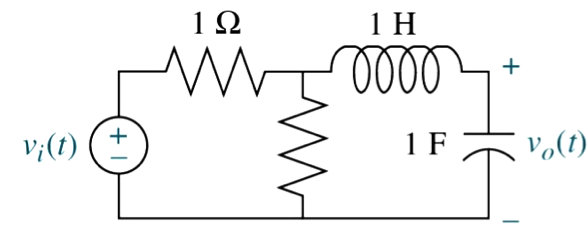
\includegraphics[width=0.5\textwidth]{testfig}
		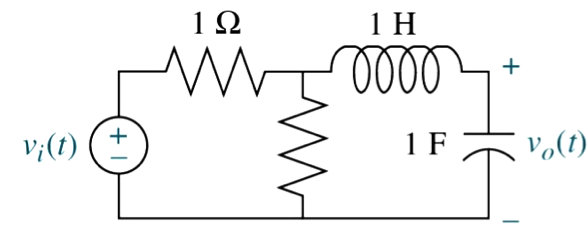
\includegraphics{testfig}
		\caption{\rajah}
		\label{fig:meshcircuit}
	\end{figure}

	% Table generated by Excel2LaTeX from sheet 'Sheet1'
	\begin{table}[H]
		\centering
		\caption{\jadual}
		\begin{tabular}{cc}
			\toprule
			\multicolumn{1}{l}{\textbf{Frequency}} & \multicolumn{1}{l}{\textbf{Impedance (Magnitude) ($\Omega$)}} \\
			\midrule
			5 Hz  & 20,000 \\
			10 Hz & 19,998 \\
			\vdots     & \vdots \\
			40 kHz & 602 \\
			50 kHz & 600 \\
			100 kHz & 600 \\
			\bottomrule
		\end{tabular}%
		\label{table:freqmag}%
	\end{table}%
\listclose % close 1st level question



% PART B
\clearpage	% start new page
\newpartenx{Answer any THREE (3) questions} 

\newpartbm{Jawab mana-mana TIGA (3) soalan}
\bigskip

% Question 2
\question

% question without enumerate list
Silver/silver chloride (Ag/AgCl) electrodes are commonly used in biological measurement.

\translation{Elektrod Argentum/Argentum chloride (Ag/AgCl) digunakan secara meluas didalam pengukuran biologi}	

\qmarks{5}

\listbegin	% start 1st level question
	\item \label{halfmembrane} State the definition of half-membrane
	
	\translation{Nyatakan definisi separuh-membran}
	
	\qmarks{2}
	
	\item \label{itm:net} Elaborate the basic mechanisms that contribute to condition in \ref{halfmembrane}, and write its net potential. % use label to reference to the list item
	
	\translation{Kembangkan mekanisma asas yang menyumbang kepada keadaan di \ref{halfmembrane}, dan tuliskan upaya bersih.}
	
	\qmarks{4}

	\listbegin % start 2nd level question
		\item \label{itm:ref2nd} Second level item that refer to \ref{itm:net}. Second level item. second level item. 
		
		\translation{ini adalah level kedua. ini adalah level kedua. ini adalah level kedua.} 
		
		\item Another second level that refer to \ref{itm:ref2nd}. Another second level. Another second level.
		
		\translation{ini adalah level kedua. ini adalah level kedua. ini adalah level kedua.} 
		
		\item Another second level that refer to \ref{itm:ref2nd}. Another second level. Another second level.
		
		\translation{ini adalah level kedua. ini adalah level kedua. ini adalah level kedua.} 
		
		\item Another second level that refer to \ref{itm:ref2nd}. Another second level. Another second level.
		
		\translation{ini adalah level kedua. ini adalah level kedua. ini adalah level kedua.} 


		\listbegin % start 3rd level question
			\item Another level. This is third level. This is third level. This is third level. This is third level
			
			\translation{Ini adalah level ketiga. Ini adalah level ketiga. Ini adalah level ketiga. Ini adalah level ketiga. Ini adalah level ketiga. Ini adalah level ketiga}

			\listbegin  % start 4th level question
				\item Another level. This is fourth level. This is fourth level. This is fourth level. This is fourth level. 
				
				\translation{Ini adalah level keempat. Ini adalah level keempat. Ini adalah level keempat. Ini adalah level keempat.}
			\listclose % close 4th level question
		\listclose % close 3rd level question
	\listclose % close 2nd level question
\listclose	% close 1st level question
% Question 3
\clearpage	% start new page
\question

Some questions here...


% Question 4
\clearpage	% start new page
\question

Silver/silver chloride (Ag/AgCl) electrodes are commonly used in biological measurement. 

\translation{Elektrod Argentum/Argentum chloride (Ag/AgCl) digunakan secara meluas didalam pengukuran biologi}	

\listbegin	% start 1st level question
	\item \label{halfmembrane} State the definition of half-membrane
	
	\translation{some translation here}
	
	\qmarks{2}
	
	\answer{Put answer to this question here. This answer scheme can be turned on and off by executing \texttt{answers} option. Refer to manual for explanation.
	} 
	
	\item \label{itm:net} Elaborate the basic mechanisms that contribute to condition in \ref{halfmembrane}, and write its net potential. % use label to reference to the list item
	
	\translation{some translation here}
	
	\qmarks{2}
	
	\answer{Put answer to this question here. This answer scheme can be turned on and off by executing \texttt{answers} option. Refer to manual for explanation.
	} 

	\listbegin % start 2nd level question
		\item \label{itm:ref2nd} Second level item that refer to \ref{itm:net}. Second level item. second level item. \\
		\translation{ini adalah level kedua. ini adalah level kedua. ini adalah level kedua.} 
		
		\qmarks{3}
		
		\answer{Put answer to this question here. This answer scheme can be turned on and off by executing \texttt{answers} option. Refer to manual for explanation.
		} 

		\listbegin % start 3rd level question
			\item Another level. This is third level. This is third level. This is third level. This is third level\\
			\translation{Ini adalah level ketiga. Ini adalah level ketiga. Ini adalah level ketiga. Ini adalah level ketiga. Ini adalah level ketiga. Ini adalah level ketiga.}
		\listclose % close 3rd level question
	\listclose	% close 2nd level question	
\listclose	% close 1st level question	

% Question 5
\clearpage	% start new page
\question

	\answer{ 
		This is the answer to the question 5. This answer scheme can be turned on and off by executing \texttt{answers} option. Refer to manual for explanation.
	}




\paperend

\end{document}